\section{Deployment Diagram}

\Cref{fig:implementation:deployment-diagram} shows a deployment diagram of the prototype developed during the project. Below is a brief description of each device involved in the system.

\begin{description}
\item[Smart Watch] The Motorola 360, i.e. the Android smart watch used in this project, runs the application used for creating gesture configurations and interacting with the system using gestures. We refer to this application as the \emph{CARMA app}, an abbreviation of \emph{Context AwaRe hoMe Automation}. The application stores gesture configurations in a SQLite database.
\item[BLE Beacon] the Bluetooth Low Energy beacons are used to position the user indoor. The smart watch reads the RSSI value from the Bluetooth beacons and determine which room the user is in.
\item[Raspberry Pi] The Raspberry Pi runs openHAB, which the smart watch communicates using a REST API over HTTP when loading configured beacons and rooms and when triggering actions. OpenHAB stores its data in a MapDB database, an embedded database meant to be interacted with using a Java collection framework \cite{mapdb:mapdb}.
\item[Computer] The computer runs an instance of Spotify, an application from streaming music as well as our Spotify Controls API, which allows for controlling the Spotify application over HTTP. openHAB communicates with the computer, and more specifically the API, when the user triggers an action affecting the music centre.
\item[Philips Hue Bridge] A bridge provided by Philips is installed in the users home. The bridge communicates with the Philips Hue lights using the ZigBee protocol. The protocol is described later in this section.
\item[Philips Hue Light Bulb] The light bulbs provided by Philips are controlled using gestures on the smart watch, i.e. using the CARMA application. The bulbs receive commands from the Philips Hue bridge when they need to change their state, e.g. turn on, turn off, change color or change temperature. The bulbs can communicate with each other using the ZigBee Light Link protocol to extend the range of the network by forwarding commands between bulbs.
\end{description}

In our specific prototype, we have a computer acting as the media centra and we have two Philips Hue light bulbs connected to openHAB. The number of devices will vary depending on the specific deployment, e.g. there can be more Philips Hue light bulbs or other devices in the system, e.g. door locks, a television or a thermostat.

\begin{figure}[h!]
\centering
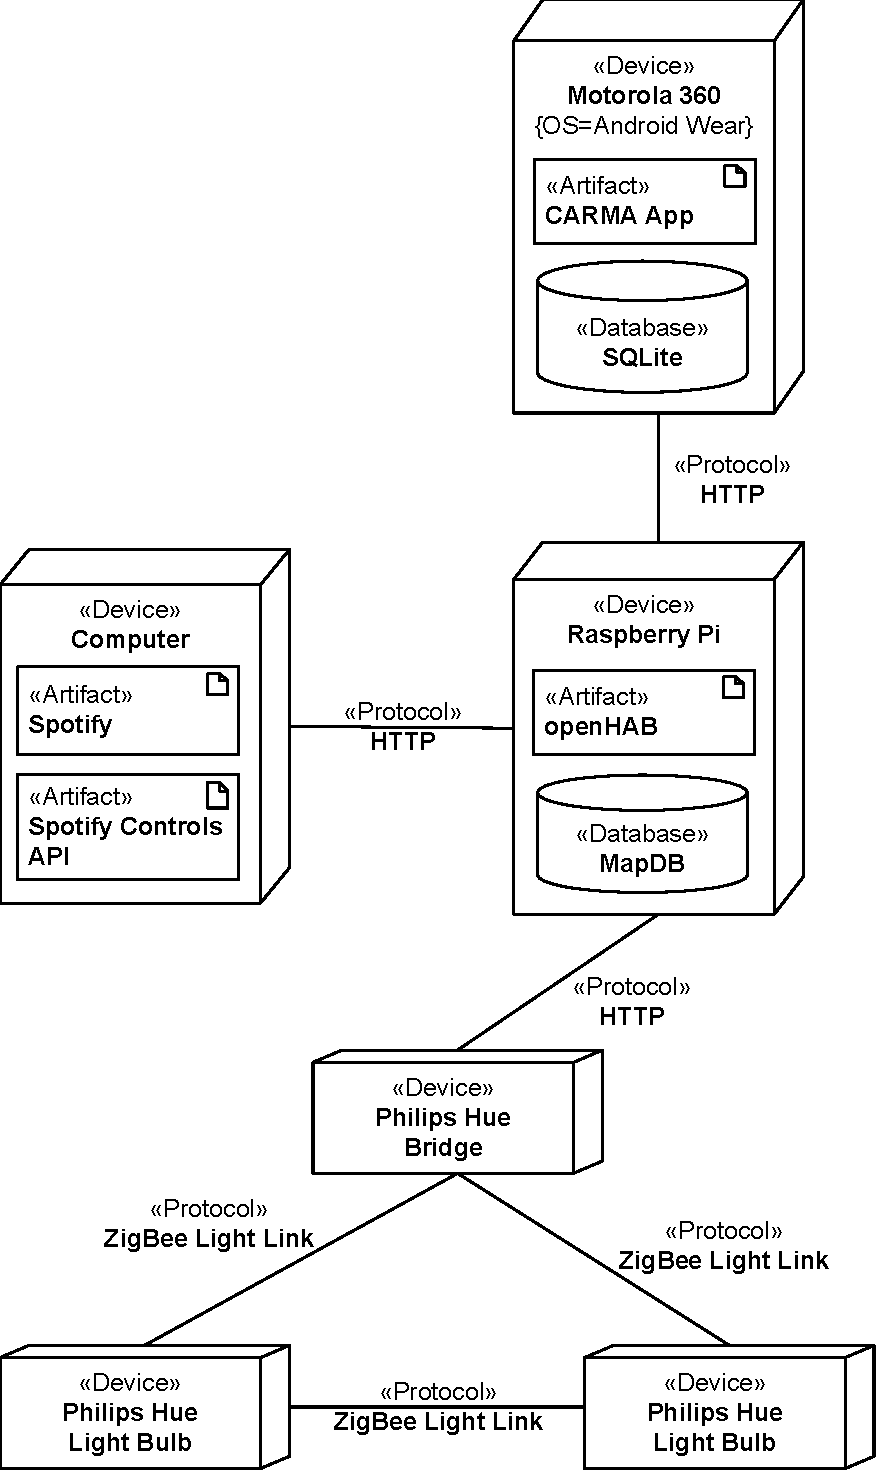
\includegraphics[height=\textheight]{images/deployment-diagram}
\caption{Deployment diagram of the prototype developed in the project.}
\label{fig:implementation:deployment-diagram}
\end{figure}

\subsection{HTTP}

HTTP, or Hyptertext Transfer Protocol, which it is short for, is a protocol amongst others used for communication between a web browser and a web server. A web browser will make a request for a specific resource and the server will return the response or a failure. In the case of a web browser, the response is typically a web page formatted as HTML which the browser can render and present to the user.

Resourecs on a web server are identified by a URL, a Uniform Resource Locator. An example of a URL is ``http://mysite.com/index.html'' which requests the ``index.html'' file on the ``mysite.com'' hostname using the ``http'' protocol.

When a web server returns a response, it will return an HTTP status code as part of the response. Examples of this includes the status code 200 for success, 404 for a resource not found and 400 for a bad request.

HTTP utilize TCP/IP to transfer information. TCP transfers information in small packets between machines and IP is responsible for addressing machines in a network and routing the information between the machines.

We use HTTP for communication between the smart watch, the Raspberry Pi and the computer acting as media centre with both expose a REST API. In the case of our prototype, we do not use a web browser to make the requests. Instead the requests are send using a framework appropriate for the platform, e.g. in the case of the smart watch application we use the Android Volley framework for making requests\footnote{For more information about Google Volley, please refer to \url{https://developer.android.com/training/volley/}}.
The requests are sent to either openHAB or the Spotify Controls API which will return a response formatted using JSON. In the case of a simple request, e.g. for changing the state of the music centre, the JSON response, as well as the HTTP status code, indicates whether or not the request was successful. For a more complex request, e.g. when requesting the available items in openHAB, the response will contain all available items in openHAB formatted as JSON along with a HTTP status code.

\subsection{ZigBee}

The ZigBee protocol is targeted towards devices that fit within the concept of internet of things, e.g. lamps, thermostats and door locks. The devices create a \emph{mesh network}, i.e. a network in which nodes relays information to other nodes \cite{zigbee:zigbee-pro}. This is depicted in the deployment diagram shown in \cref{fig:implementation:deployment-diagram} in which both Philips Hue light bulbs receives commands by the bridge but the bulbs can also relay commands to each other.

The ZigBee protocol, amongst others, specifies the frequencies on which the devices shuld communicate, how devices are discovered and how they are paired with each other.

The Philips Hue light bulbs used in our prototype utilize the ZigBee Light Link standard, an extension of the ZigBee protocol, which is a ZigBee standardization of how communication with light bulbs is done, e.g. the information sent to the bulbs when changing their state.

In this project, we have not implemented communication using ZigBee, but instead utilize HTTP to communiate with the Philips Hue brdige which in turn communicates with the bulbs using the ZigBee protocol.

%%% Local Variables:
%%% mode: latex
%%% TeX-master: "../../master"
%%% End:
